\documentclass[11pt]{beamer}
\graphicspath{{img/}{./}}
\usepackage[french]{babel}
\usepackage{graphicx}
\usepackage{ulem} %Pour biffer du texte \sout{texte barré}
\usepackage{xcolor} 
\usepackage{tabularx}
\usepackage{parallel}
%\usepackage[babelshorthands]{polyglossia}
\usepackage{ragged2e} 


%Allignemebnt droite/gauche
\usepackage{polyglossia}
%\usepackage[babelshorthands]{polyglossia} %[babelshorthands] permet d'avoir les guillemets allemands avec le code "`toto"' et les guillemets français avec le code "<tata">


\usepackage{multirow} 
\setmainlanguage{english}
\usepackage[autostyle]{csquotes}
\MakeOuterQuote{"}
\DeclareQuoteStyle{english}%
    {\textquotedblleft}
    [\textquotedblleft]
    {\textquotedblright}
        [0.05em]
    {\textquoteleft}
    [\textquoteleft]
    {\textquoteright}
% \DeclareQuoteStyle[quotes]{french}
%   {\mkfrenchopenquote{«}}
%   {\mkfrenchclosequote{\nobreakspace»}}
%   {\textquotedblleft}
%   {\textquotedblright}
% \DeclareQuoteStyle[quotes*]{french}
%   {\mkfrenchopenquote{«}}
%   {\mkfrenchclosequote{\nobreakspace»}}
%   {\mkfrenchopenquote{\textquotedblleft}}
%   {\mkfrenchclosequote{\textquotedblright}}
% \DeclareQuoteStyle[guillemets]{french}
%   [\initfrenchquotes]
%   {\mkfrenchopenquote{«}}
%   [\mkfrenchopenquote{«}]
%   {\mkfrenchclosequote{\nobreakspace»}}
%   {\mkfrenchopenquote{«}}
%   [\mkfrenchopenquote{«}]
%   {\mkfrenchclosequote{\nobreakspace»}}
% \DeclareQuoteStyle[guillemets*]{french}
%   [\initfrenchquotes]
%   {\mkfrenchopenquote{«}}
%   [\mkfrenchopenquote{\nobreakspace»}]
%   {\mkfrenchclosequote{\nobreakspace»}}
%   {\mkfrenchopenquote{«}}
%   [\mkfrenchopenquote{\nobreakspace»}]
%   {\mkfrenchclosequote{\nobreakspace»}}




\setotherlanguage{greek}
\newfontfamily\greekfont[Script=Greek]{Linux Libertine O}
\newfontfamily\greekfontsf[Script=Greek]{Linux Libertine O}
\setotherlanguage{hebrew}
\newfontfamily{\hebrewfont}[Script=Hebrew, Path=./fonts/]{SBL_Hbrw.ttf}
\newfontfamily{\hebrewfontsf}[Script=Hebrew]{Miriam CLM}
\newfontfamily{\hebrewfonttt}[Script=Hebrew]{Miriam Mono CLM}
\setotherlanguage{syriac}
\newfontfamily\syriacfont[Script=Syriac, Path=./fonts/]{EstrangeloEdessa.ttf}

\usepackage{booktabs} % Allows the use of \toprule, \midrule and \bottomrule for better rules in tables
%% Allow the use of tcolorbox
\usepackage[skins]{tcolorbox}
%\usetheme{default}
%\usetheme{AnnArbor}
%\usetheme{Antibes}
%\usetheme{Bergen}
%\usetheme{Berkeley}
%\usetheme{Berlin}
%\usetheme{Boadilla}
%\usetheme{CambridgeUS}
%\usetheme{Copenhagen}
%\usetheme{Darmstadt}
%\usetheme{Dresden}
%\usetheme{Frankfurt}
%\usetheme{Goettingen}
%\usetheme{Hannover}
%\usetheme{Ilmenau}
\usetheme{JuanLesPins}
%\usetheme{Luebeck}
%\usetheme{Madrid}
%\usetheme{Malmoe}
%\usetheme{Marburg}
%\usetheme{Montpellier}
%\usetheme{PaloAlto}
%\usetheme{Pittsburgh}
%\usetheme{Rochester}
%\usetheme{Singapore}
%\usetheme{Szeged}
%\usetheme{Warsaw}

%----------------------------------------------------------------------------------------
%	SELECT COLOR THEME
%----------------------------------------------------------------------------------------

% Beamer comes with a number of color themes that can be applied to any layout theme to change its colors. Uncomment each of these in turn to see how they change the colors of your selected layout theme.

%\usecolortheme{albatross}
%\usecolortheme{beaver}
%\usecolortheme{beetle}
%\usecolortheme{crane}
%\usecolortheme{dolphin}
%\usecolortheme{dove}
%\usecolortheme{fly}
%\usecolortheme{lily}
%\usecolortheme{monarca}
%\usecolortheme{seagull}
%\usecolortheme{seahorse}
%\usecolortheme{spruce}
%\usecolortheme{whale}
%\usecolortheme{wolverine}

%----------------------------------------------------------------------------------------
%	SELECT FONT THEME & FONTS
%----------------------------------------------------------------------------------------
\setmainfont{cochineal}
% Beamer comes with several font themes to easily change the fonts used in various parts of the presentation. Review the comments beside each one to decide if you would like to use it. Note that additional options can be specified for several of these font themes, consult the beamer documentation for more information.

%\usefonttheme{default} % Typeset using the default sans serif font
\usefonttheme{serif} % Typeset using the default serif font (make sure a sans font isn't being set as the default font if you use this option!)
%\usefonttheme{structurebold} % Typeset important structure text (titles, headlines, footlines, sidebar, etc) in bold
%\usefonttheme{structureitalicserif} % Typeset important structure text (titles, headlines, footlines, sidebar, etc) in italic serif
%\usefonttheme{structuresmallcapsserif} % Typeset important structure text (titles, headlines, footlines, sidebar, etc) in small caps serif

%------------------------------------------------

%\usepackage{mathptmx} % Use the Times font for serif text
%\usepackage{palatino} % Use the Palatino font for serif text


%\usepackage{helvet} % Use the Helvetica font for sans serif text
%\usepackage[default]{opensans} % Use the Open Sans font for sans serif text
%\usepackage[default]{FiraSans} % Use the Fira Sans font for sans serif text
%\usepackage[default]{lato} % Use the Lato font for sans serif text

%----------------------------------------------------------------------------------------
%	SELECT INNER THEME
%----------------------------------------------------------------------------------------

% Inner themes change the styling of internal slide elements, for example: bullet points, blocks, bibliography entries, title pages, theorems, etc. Uncomment each theme in turn to see what changes it makes to your presentation.

%\useinnertheme{default}
%\useinnertheme{circles}
\useinnertheme{rectangles}
%\useinnertheme{rounded}
%\useinnertheme{inmargin}

%----------------------------------------------------------------------------------------
%	SELECT OUTER THEME
%----------------------------------------------------------------------------------------

% Outer themes change the overall layout of slides, such as: header and footer lines, sidebars and slide titles. Uncomment each theme in turn to see what changes it makes to your presentation.

%\useoutertheme{default}
%\useoutertheme{infolines}
%\useoutertheme{miniframes}
%\useoutertheme{smoothbars}
%\useoutertheme{sidebar}
%\useoutertheme{split}
%\useoutertheme{shadow}
%\useoutertheme{tree}
%\useoutertheme{smoothtree}

%\setbeamertemplate{footline} % Uncomment this line to remove the footer line in all slides
%\setbeamertemplate{footline}[page number] % Uncomment this line to replace the footer line in all slides with a simple slide count

%\setbeamertemplate{navigation symbols}{} % Uncomment this line to remove the navigation symbols from the bottom of all slides
\usepackage[style=sbl]{biblatex}


\DeclareSourcemap{
  \maps[datatype=bibtex]{
    \map{
      \step[fieldset=doi, null]
      \step[fieldset=language, null]
      \step[fieldset=issn, null]{}
      \step[fieldset=url, null]{}
      \step[fieldset=isbn, null]{}
      \step[fieldset=eprint, null]{}
    }
  }
}

\addbibresource{references.bib}
%\defbibheading{bibempty}{}

%----------
% Define sectioning
\AtBeginSection[]{
  \begin{frame}
  \vfill
  \centering
  \begin{beamercolorbox}[sep=8pt,center,shadow=true,rounded=true]{title}
    \usebeamerfont{title}\insertsectionhead\par%
  \end{beamercolorbox}
  \vfill
  \end{frame}
}

%-----------

%----------------------------------------------------------------------------------------
%	PRESENTATION INFORMATION
%----------------------------------------------------------------------------------------


\title{Introduction à la critique textuelle}
\author[Frédérique Michèle Rey, Sophie Robert-Hayek]{Frédérique Michèle Rey \& Sophie Robert-Hayek}


\institute[UL]{Université de Lorraine } %\smallskip \textit{frederique.rey@univ-lorraine.fr / sophie.robert@univ-lorraine.fr}}

\date{}
\usepackage[table]{xcolor}
\usepackage[dvipsnames]{xcolor}
\usepackage{forest}
\usepackage{tikz-qtree}
\usepackage[font=scriptsize]{caption}
\begin{document}
\subtitle{Session 1 : Bible hébraïque}


\begin{frame}
	\titlepage
\end{frame}

\section{Introduction}

\begin{frame}{Introduction}
\begin{block}{}
\centering Qu'est-ce que le texte biblique ?
\end{block}
\end{frame}

\begin{frame}{Quel est le texte de la bible ?}
\begin{block}{Deut 32:8}
\RTL\noindent
\texthebrew{בְּהַנְחֵל עֶלְיוֹן גּוֹיִם בְּהַפְרִידוֹ בְּנֵי אָדָם יַצֵּב גְּבֻלֹת עַמִּים לְמִסְפַּר בְּנֵי יִשְׂרָאֵֽל׃}
\end{block}

\pause

\begin{exampleblock}{Traduction de Louis Segond (1910)}
Quand le Très-Haut donna un héritage aux nations, Quand il sépara les enfants des hommes, Il fixa les limites des peuples D'après le nombre des \textbf{\textcolor{red}{enfants d'Israël}}.  
\end{exampleblock}

\pause

\begin{alertblock}{Traduction de la Bible de Jérusalem}
Quand le Très Haut donna aux nations leur héritage, quand il répartit les fils d'homme, il fixa les limites des peuples suivant le nombre des \textbf{\textcolor{red}{fils de Dieu}}.
\end{alertblock}
    
\end{frame}

\begin{frame}{Quel est le texte de la bible ?}
    \begin{figure}
        \centering
        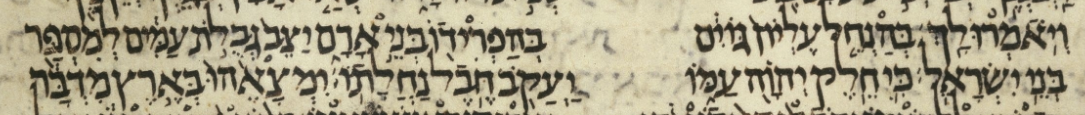
\includegraphics[width=1\linewidth]{img/leningrad_deut_32_8.png}
        \caption{Deut 32:8 dans le Codex de Leningrad (Xe siècle)}
    \end{figure}
    \begin{block}{\RTL \texthebrew{בְּהַנְחֵל עֶלְיוֹן גּוֹיִם בְּהַפְרִידוֹ בְּנֵי אָדָם יַצֵּב גְּבֻלֹת עַמִּים לְמִסְפַּר בְּנֵי יִשְׂרָאֵֽל׃}}
       
        Quand le Très-Haut donna un héritage aux nations, Quand il sépara les enfants des hommes, Il fixa les limites des peuples D'après le nombre des \textbf{\textcolor{red}{enfants d'Israël}}.
    \end{block}
\end{frame}

\begin{frame}{Quel est le texte de la bible ?}
    \begin{figure}
        \centering
        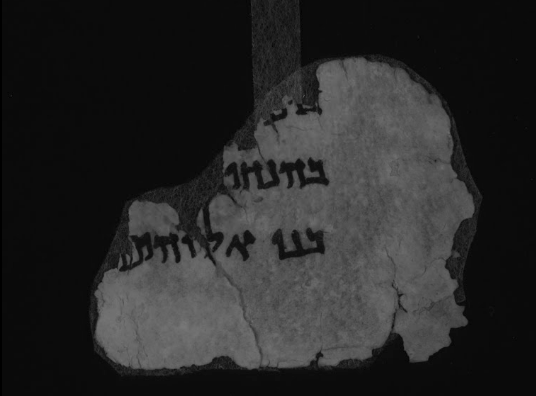
\includegraphics[width=.5\linewidth]{img/4Q37_12_deut_32_8.png}
        \caption{Deut 32:8 dans 4Q37 (Ier siècle avant notre ère)}
    \end{figure}
    \begin{alertblock}{\RTL \texthebrew{בהנחל[ עליון גוים בהפרידו בני אדם יצב גבלת עמים למספר] בני אלוהים}}
        Quand le Très-Haut donna un héritage aux nations, Quand il sépara les enfants des hommes, Il fixa les limites des peuples D'après le nombre des \textbf{\textcolor{red}{enfants de Dieu}}.
    \end{alertblock}
\end{frame}

\begin{frame}{Quel est le texte de la bible ?}
    \begin{alertblock}{La Septante}
        \textgreek{ὅτε διεμέριζεν ὁ ὕψιστος ἔθνη, ὡς διέσπειρεν υἱοὺς Αδαμ, ἔστησεν ὅρια ἐθνῶν κατὰ ἀριθμὸν ἀγγέλων θεοῦ}\\
        
        Quand le Très-Haut a dispersé les nations, Quand il a disséminé les enfants d'Adam, Il a établi les les frontières des nations selon le nombre des \textbf{\textcolor{red}{anges de Dieu}}.
    \end{alertblock}
\end{frame}

\begin{frame}{Quel est le VRAI texte ?}
\begin{block}{Une double vérité}
\pause
\begin{columns}
    \column{0.4\textwidth}
        \centering
        \begin{alertblock}{}
        \centering La vérité du document
        \end{alertblock}
    \column{0.3\textwidth}
        \centering
        \begin{exampleblock}{}
        \centering La vérité de l'auteur
        \end{exampleblock}
\end{columns}
\end{block}
\tiny{Voir \fullcite{avalle_doppia_2002}}
\end{frame}


\begin{frame}{Plan du cours}
\begin{itemize}
    \item La critique textuelle. Une petite histoire de la philologie
    \item Les témoins manuscrits de l'Ancien Testament
    \item Petit manuel d'utilisation d'une édition critique de la bible hébraïque
    \item "Éloge de la variante"
    \item Cas d'étude
\end{itemize}
\end{frame}

\end{document}